\documentclass[14pt,a4paper]{extreport}
\usepackage[utf8]{inputenc}
\usepackage[english]{babel}
\usepackage{amsmath}
\usepackage{amsfonts}
\usepackage{amssymb}
\usepackage{graphicx}
\usepackage{titlesec}
\usepackage{caption}
\usepackage{subcaption}
\usepackage{float}
\usepackage[export]{adjustbox}
\graphicspath{ {data/} }
\titleformat{\chapter}[display]
  {\Huge\bfseries}
  {}
  {0pt}
  {\thechapter.\ }

\titleformat{name=\chapter,numberless}[display]
  {\Huge\bfseries}
  {}
  {0pt}
  {}
\usepackage[left=3cm,right=3cm,top=3cm,bottom=3cm]
{geometry}
\title{Gaze detection}
\date{Final Computer Vision Project\\ September 2019}
\author{Giovanni Gallinaro}
\begin{document}
\maketitle

The goal of this work is to write a C++ program exploiting opencv in Microsoft Visual Studio which is able to detect the direction of the gaze of a person in a picture. The program will read in input a certain number of images and will return as output the direction of the gaze of each person in the pictures as RIGHT, LEFT or STRAIGHT; the direction is related to the viewpoint of the person in the picture.

The main idea behind the project is to detect the iris/pupil and compute its position related to the horizontal corners of the sclera of the eye in order to establish the direction of the gaze.

The program firstly reads in input the images and stores them in a vector of Mat elements. Each one of them is then iterated in order to process each image indipendently. In this report I will refer to a single image but the same procedure is applied to all the others.

First of all the features related to the faces in the image are detected by using an Haar Feature-based Cascade Classifier. This is done by function \textit{detect}\_\textit{features}, which loads the classifier for face recognition from the opencv folder: in particular, the \textit{haarcascade}\_\textit{frontalface}\_\textit{alt.xml} has been used for this project since it gives better results. The regions of the faces are represented as rectangles which are drawn on the original image to show the results of the detection. Also the relevant coordinates of the rectangles are stored into an array which is then given in output. The detection of the eyes is instead computed inside the region of each face by means of the same procedure (as seen for the faces extraction from the original image). The regions related to the eyes are organized in a bi-dimensional vector in which the first index indicates the face and the second index contains all the eyes associated to that particular face. Figure \ref{fig:feature} shows the result of such detection.

\begin{figure}[h]
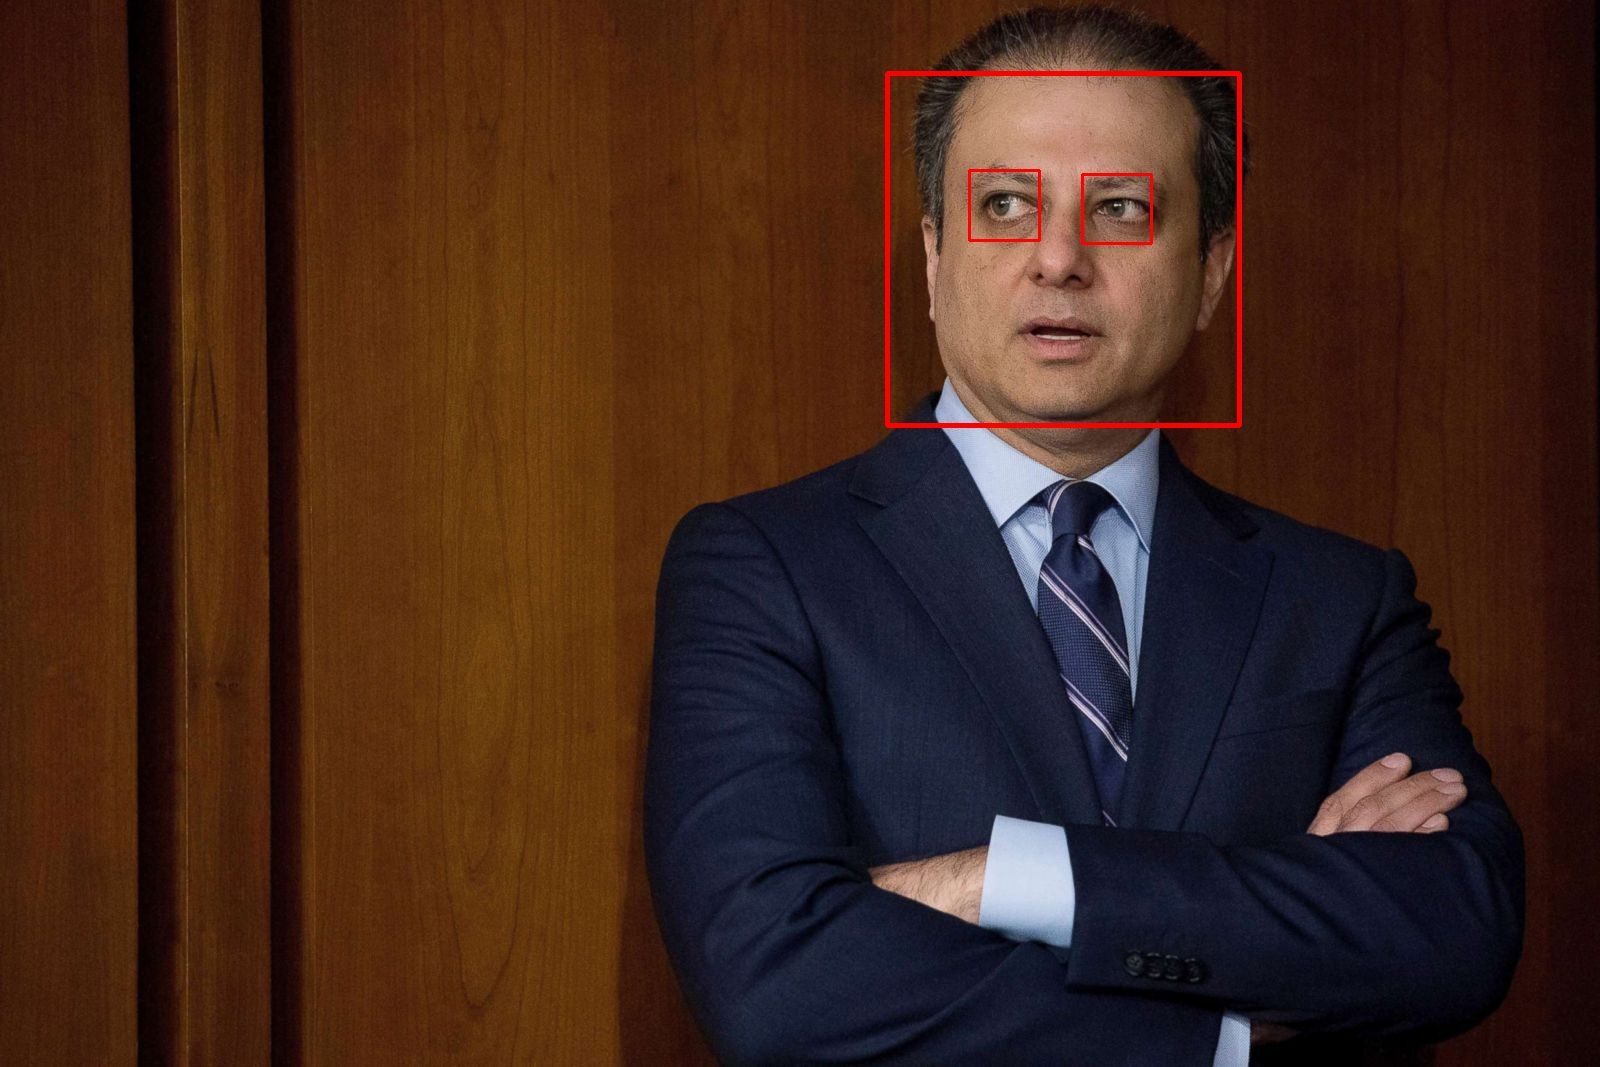
\includegraphics[width=\linewidth, center]{images_T2S/0_features.jpg} 
\caption{Feature Detection.}
\label{fig:feature}
\end{figure}

Subsequently, the detected eyes are cropped from the original image in order to process them separately. Before moving to the detection of the iris and corners, the cropped images are pre-processed: each of them is converted to gray-scale color space and then the constrast is amplified in order to better distinguish the dark regions from the light ones. 

The goal is to obtain a segmented binary image that well highlights the region corresponding to the iris by applying a threshold that keeps only the darker regions. To do so, the threshold is computed individually for each image in order to obtain a segmentation that best represents the corresponding eye. We notice that lighter images require a higher threshold in order to obtain better results. The amount of light present in the picture is measured by computing a weighted average of the histogram values where the weight is the intensity. The threshold value is a quantized version the return value of the average. In Figure \ref{fig:thresh} the segmentation has been applied with the computed threshold value of 150.

\begin{figure}[h]

\includegraphics[width=0.5\linewidth, center]{images_T2S/5_bin_eye0.jpg} 
\caption{Binary Segmentation.}
\label{fig:thresh}
\end{figure}

In order to detect the region corresponding to the iris the program computes the barycenter of the black cluster. For a more precise result, the barycenters are computed on multiple segmented images with different thresholds varying within a range around the ideal one (similarly to the Watershed algorithm for what concerns the multiple thresholding technique). The output is shown in Figure \ref{fig:centr} and consists in taking the average coordinates between the centroids obtained by the multiple thresholding.

\begin{figure}[h]
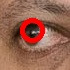
\includegraphics[width=0.5\linewidth, center]{images_T2S/5_centroid0.jpg} 
\caption{Centroid computed from the Multiple Thresholding.}
\label{fig:centr}
\end{figure}

The edges of the sclera are computed in a similiar manner: for each thresholded image the minimum and maximum values of the x coordinate of the points belonging to the black region are computed. The final outcomes are taken by averaging these values. The results are shown Figure \ref{fig:extr}.

\begin{figure}[h]
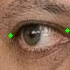
\includegraphics[width=0.5\linewidth, center]{images_T2S/5_extr0.jpg} 
\caption{Extremes of the sclera.}
\label{fig:extr}
\end{figure}

Finally, the distance between the iris and both corners of the sclera is computed and the direction is determinated in the following way:

\begin{itemize}
	\item If the distance from the iris and the left corner is less than 45\% of the distance between the two corners, the value RIGHT is assigned.
	\item If the distance from the iris and the left corner is more than 55\% of the distance between the two corners, the value LEFT is assigned.
	\item Otherwise, STRAIGHT is assigned.
\end{itemize}

Figure \ref{fig:final} shows the final output of the program.

\begin{figure}[h]
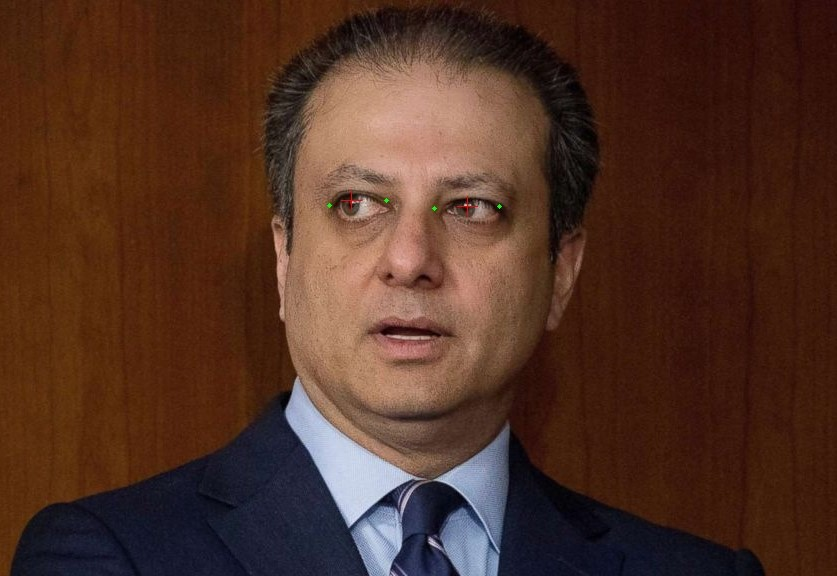
\includegraphics[width=\linewidth, center]{images_T2S/5_final0.jpg} 
\caption{Final output.}
\label{fig:final}
\end{figure}

\end{document}